%%% ====================================================================
%%% Início da parte textual do documento.


%%% Configuração do espaçamento entre títulos e texto
\setlength{\afterchapskip}{1.5cm minus \baselineskip}


\chapter{Metodologia}
\label{cha:metodologia}

\section{Arquitetura utilizada}

\subsection{Componentes}

Para elaboração do sistema proposto, foi utilizado uma arquitetura baseada em sistemas distribuídos, que a partir do protocolo HTTP comunica-se entre seus componentes. Esses componentes podem ser vistos na figura \ref{fig:arquitetura}:

\begin{figure}[H]
	\centering
	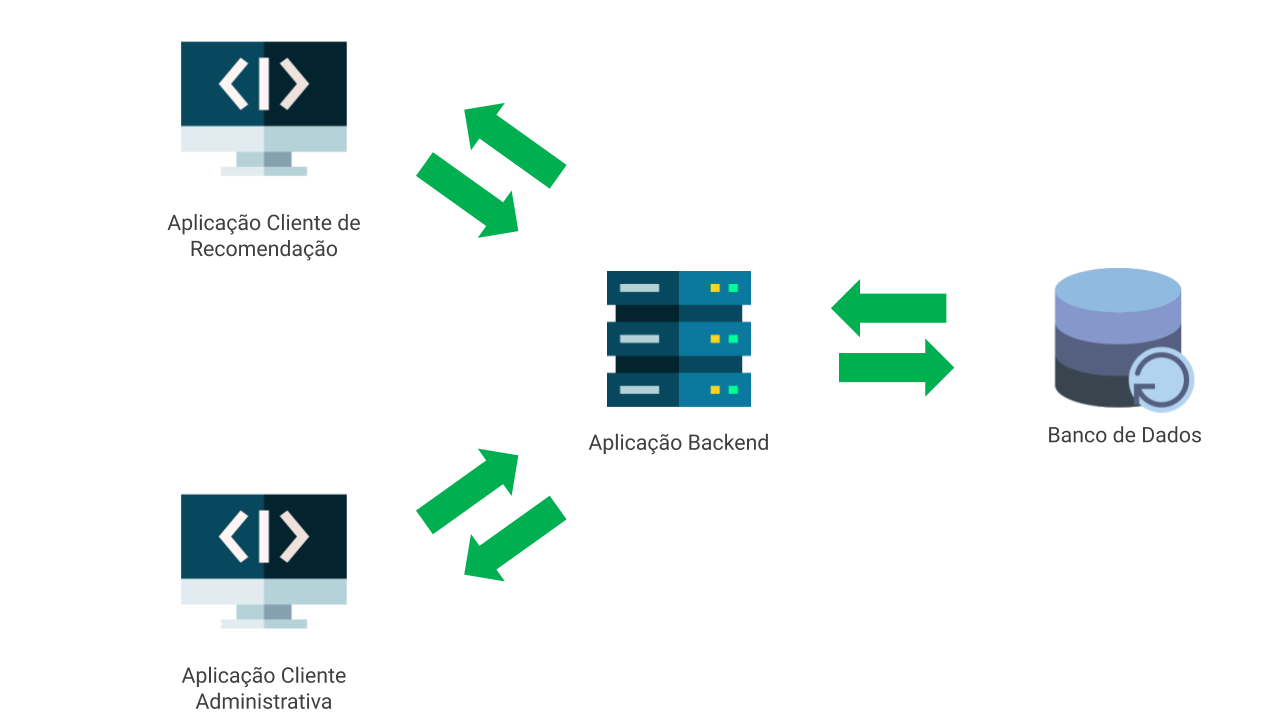
\includegraphics[width=0.7\linewidth]{imagens/arquitetura.png}
	\caption[Arquitetura do sistema]{Arquitetura do sistema (AUTOR, 2020)}
    \label{fig:arquitetura}
\end{figure}

Cada um dos componentes definidos apresenta uma respectiva função no sistema, que pode ser observada abaixo:

\begin{itemize}
    \item \textbf{Backend:} responsável pelo processamento e gerenciamento das recomendações e de todos os recursos existentes no sistema.
    
    \item \textbf{Cliente Administrativo:} aplicação gráfica para acesso e manipulação dos recursos pelo administrador do sistema. Nessa aplicação o administrador poderá manipular os recursos relacionados aos seus casos de uso além de poder emitir diversas listagens e relatórios para avaliação dos resultados gerados pelo sistema.
    
    \item \textbf{Cliente de Recomendação:} aplicação gráfica para acesso e manipulação dos recursos pelos avaliadores do sistema.
\end{itemize}

\subsection{Tecnologias}

As seguintes tecnologias foram utilizadas para elaboração do sistema:

\begin{itemize}
    \item \textbf{Java 14:} linguagem escolhida para desenvolvimento do backend devido a facilidade de implementação de concorrência e por ter sido utilizada na elaboração dos algoritmos usados como base para elaboração do sistema proposto.
    
    \item \textbf{Spring Boot 2.2.6:} framework utilizado para desenvolvimento da arquitetura web do backend. Possui diversas bibliotecas e implementações que facilitam o desenvolvimento de sistemas robustos e seguros.
    
    \item \textbf{PostgreSQL:} sistema de banco de dados que utiliza a especificação SQL em seu funcionamento.
    
    \item \textbf{H2:} sistema de banco de dados em memória utilizado para testes da aplicação.
    
    \item \textbf{VueJS:} Framework web baseado em Javascript, possui diversas ferramentas e recursos que facilitam o processo de desenvolvimento. 
    
    \item \textbf{Quasar Framework:} biblioteca baseada no VueJS que dispõe inúmeros componentes e estruturas para desenvolvimento de sistemas web com alta performance. Utilizado para desenvolvimento dos clientes frontend do sistema.
    
    \item \textbf{JWT:} especificação para transferência segura de dados a partir de requisições HTTP, definida na RFC 7519 \cite{ietftools}. Segundo \citeonline{jones2015json}, o JWT apresenta-se como uma alternativa concreta para transmissão de informações confidenciais em sistemas stateless.
\end{itemize}


\subsection{Ferramentas}

No processo de desenvolvimento do sistema proposto, foram utilizadas as seguintes ferramentas:

\begin{itemize}
    \item \textbf{IntelliJ IDEA Community:} IDE utilizada para desenvolvimento do backend da aplicação e gerenciamento de suas dependências.

    \item \textbf{PhpStorm:} IDE utilizada para desenvolvimento dos clientes frontend e gerenciamento de suas dependências.

    \item \textbf{Git e Github:} Ferramentas utilizadas respectivamente no versionamento e na criação e publicação dos repositórios na internet.

    \item \textbf{pgAdmin4:} ferramenta gráfica para manipulação e gerenciamento do banco de dados PostgreSQL.
    
    \item \textbf{Postman:} ferramenta utilizada para realização de requisições HTTP para o sistema e na geração de documentação para a API.

    \item \textbf{Adobe XD:} ferramenta utilizada para criação dos protótipos e wireframes dos clientes frontend do sistema.

    \item \textbf{Docker e Docker Compose:} ferramentas baseadas em containers e utilizadas na criação do banco de dados PostgreSQL e na ferramenta pgAdmin4, possibilitando uma melhor interoperabilidade entre diversos sistemas operacionais.
    
    \item \textbf{UML (Unified Modeling Language):} ferramenta para modelagem do sistema, que segundo \citeonline{booch2006uml}, pode ser definida como uma linguagem gráfica utilizada para visualização, construção, especificação e documentação de artefatos em sistemas de software complexos.
    
    \item \textbf{Astah Community:} ferramenta utilizada na criação dos diagramas UML para documentação do backend do sistema.
    
    \item \textbf{Git Flow:} ferramenta utilizada para organização e fluxo dos versionamentos de código. O modelo apresentado pelo Git Flow permite aos desenvolvedores um maior controle das ramificações \textit{(branch)} e fluxos de trabalho criados no Git, organizando e separando controle de recursos, hotfixes \footnote{Mudanças de código pontuais, normalmente utilizadas para correções de bugs \cite{chopra2014automated}} e versões em softwares de maior escala \cite{kreeftmeijer2015using}.
\end{itemize}

\section{Algoritmo}

Para desenvolvimento dos algoritmos de filtragem colaborativa e baseada em conteúdo, foram usados como base, respectivamente, os trabalhos de \citeonline{tcctiago} e \citeonline{tccluisa}. A recomendação híbrida combina os dois métodos de recomendações (colaborativa e baseada em conteúdo) e gera seus resultados de acordo com a abordagem definida para execução do algoritmo. Todos os cálculos podem serem vistos detalhadamente na seção de Anexos desse trabalho.

\subsection{Distância euclidiana}

O cálculo da distância euclidiana prove a medição da distância entre dois pontos, permitindo desse modo, sua utilização para definição da similaridade entre os objetos de um sistema de recomendação. A fórmula da distância euclidiana pode ser visualizada abaixo:

\begin{equation*}
    DE\left( x,y\right)   = \sqrt {\sum _{i}^{p}  \left( x_{i}-y_{i}\right)^2 }
    \label{eq:euclidiana}
\end{equation*}

\subsection{Recomendação colaborativa}

Para exemplificação do algoritmo de filtragem colaborativa, será utilizado o exemplo apresentado na figura \ref{fig:algoritmocolaborativo}:

\begin{figure}[H]
	\centering
	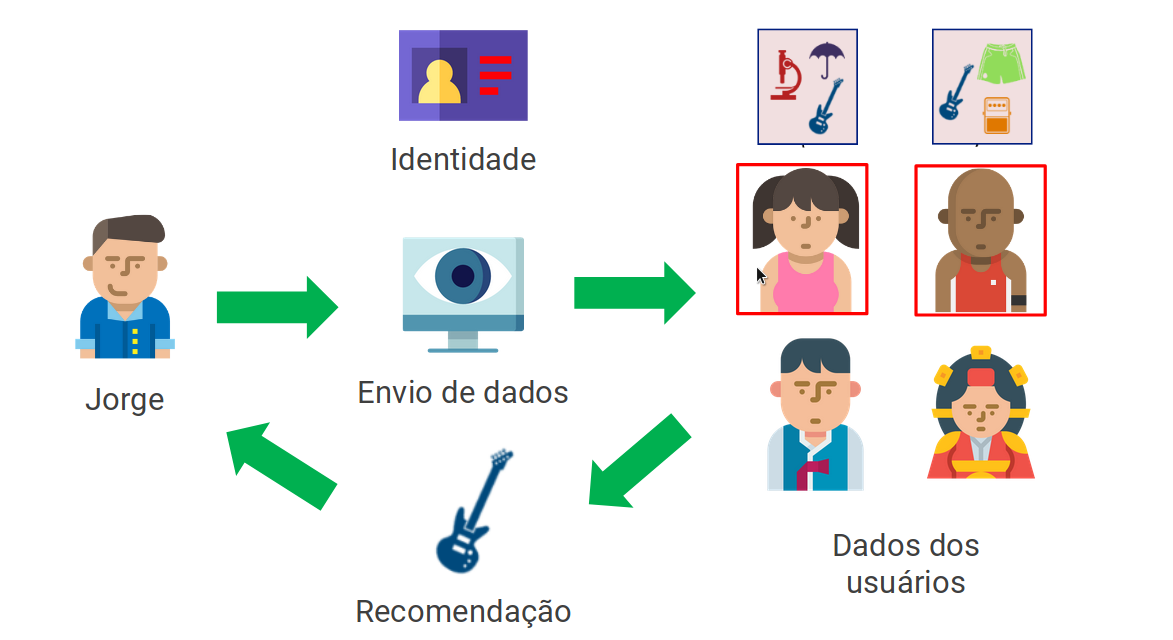
\includegraphics[width=0.7\linewidth]{imagens/colaborativa.png}
	\caption[Exemplo de filtragem colaborativa]{Exemplo de filtragem colaborativa, adaptado de \cite{araujo2011apprecommender}}
    \label{fig:algoritmocolaborativo}
\end{figure}

No seguinte exemplo, têm-se um usuário (definido como Jorge) que está acessando um site de vendas que possui um sistema de recomendação baseado em conteúdo. Durante o acesso de Jorge ao site, o sistema realiza uma coleta e análise de seus dados de navegação, procurando traçar o seu perfil de usuário (representado como a identidade na figura \ref{fig:algoritmocolaborativo}). Esse perfil é utilizado para quantificação e análise da avaliação do Jorge acerca dos produtos do site.

A partir da comparação do perfil do Jorge com o de outros usuários, é possível definir um vínculo de similaridade entre os perfis de ambos. Com isso, é possível identificar quais os usuários com os gostos mais parecidos com o Jorge, esses usuários são identificados como vizinhos.

Com a análise dos perfis dos vizinhos, torna-se possível identificar quais seriam os prováveis itens que poderiam ser recomendados ao Jorge, levando em conta que provavelmente os itens comprados pelos vizinhos atendem ao gosto do Jorge. 

\subsection{Recomendação baseada em conteúdo}

Para exemplificação do algoritmo de filtragem baseada em conteúdo, será utilizado o exemplo apresentado na figura \ref{fig:algoritmoconteudo}:

\begin{figure}[H]
	\centering
	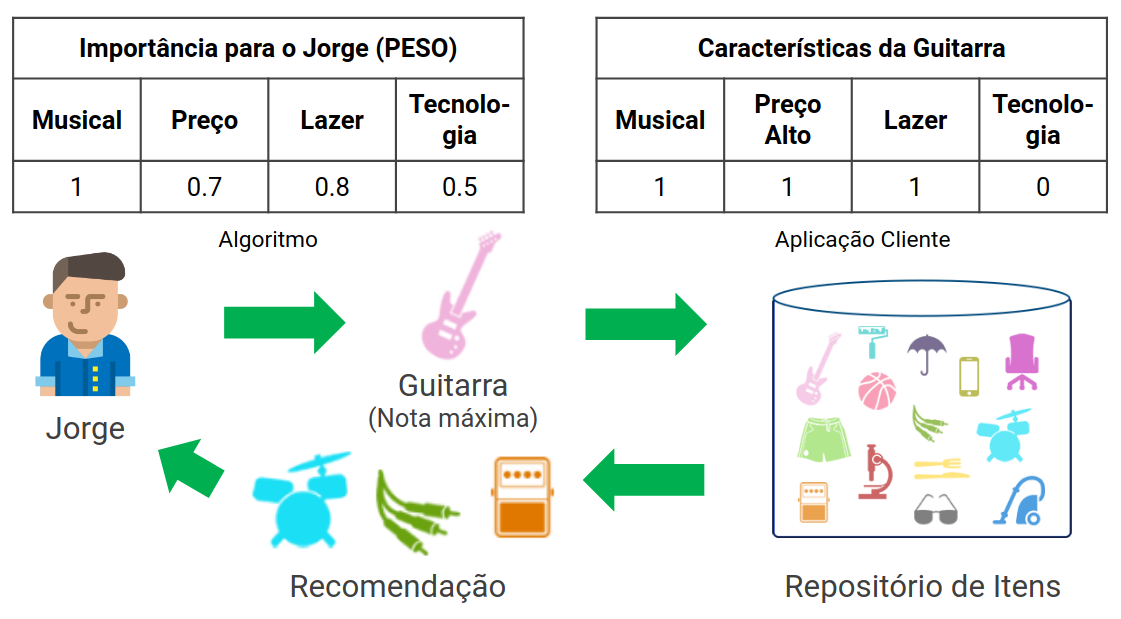
\includegraphics[width=0.7\linewidth]{imagens/baseadoconteudo.png}
	\caption[Exemplo de filtragem baseada em conteúdo]{Exemplo de filtragem baseada em conteúdo, adaptado de \cite{araujo2011apprecommender}}
    \label{fig:algoritmoconteudo}
\end{figure}

No seguinte exemplo, temos o mesmo caso apresentado no algoritmo de filtragem colaborativa, contudo utilizando a abordagem de recomendação baseada em conteúdo.

No caso apresentado, o usuário Jorge realiza a compra de uma guitarra em um site de compras que está utilizando a abordagem baseada em conteúdo para recomendação de produtos. Nesse modelo de produto, foram definidos algumas tags que possuem uma nota que define o quanto o produto atende a característica definida na tag em questão (tabela de características da guitarra).

A partir dessa tabela de característica, somada a dos outros produtos que Jorge possa ter comprado ou avaliado, é possível gerar uma tabela de importância das tags para o Jorge, que definirá quais os atributos que ele considera mais importantes na compra de um produto.

Com essa tabela gerada, é possível utilizá-la para multiplicação e geração dos pesos que Jorge possivelmente dará aos produtos ainda não avaliados. Logo, torna-se possível recomendar os itens que possuam as melhores notas.

\subsection{Recomendação Híbrida}

Na recomendação híbrida é utilizado uma combinação das abordagens colaborativa e baseada em conteúdo conforme a figura \ref{fig:algoritmohibrido}:

\begin{figure}[H]
	\centering
	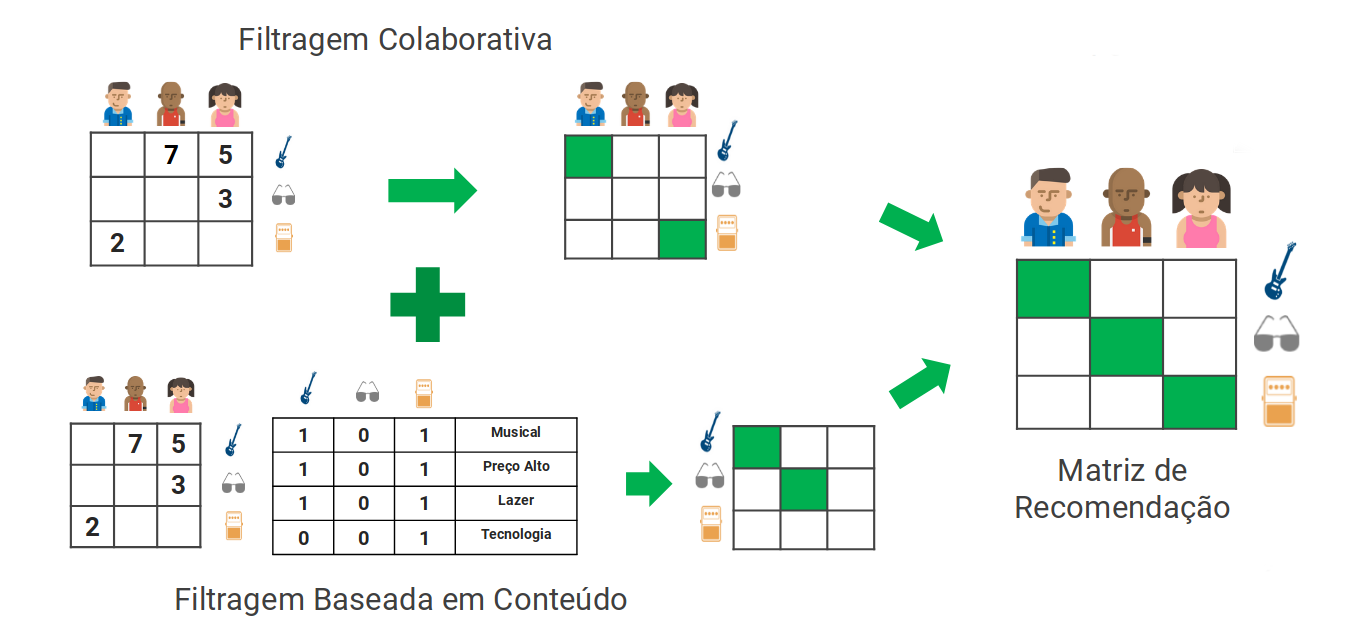
\includegraphics[width=1\linewidth]{imagens/hibrida.png}
	\caption[Exemplo de filtragem híbrida]{Exemplo de filtragem híbrida, adaptado de \cite{araujo2011apprecommender}}
    \label{fig:algoritmohibrido}
\end{figure}

A partir dos resultados gerados em cada uma das abordagens é possível realizar um processo que gere um valor final para a matriz que será recomendada, sendo que, esse processo irá variar de acordo com a abordagem escolhida. 

No trabalho apresentado estão sendo utilizadas as abordagens mista e ponderada para recomendação híbrida.

Na abordagem mista os resultados gerados por ambas as recomendações (colaborativa e baseada em conteúdo) são enviados para o cliente que solicitou a recomendação, conforme figura \ref{fig:algoritmohibridomisto}:

\begin{figure}[H]
	\centering
	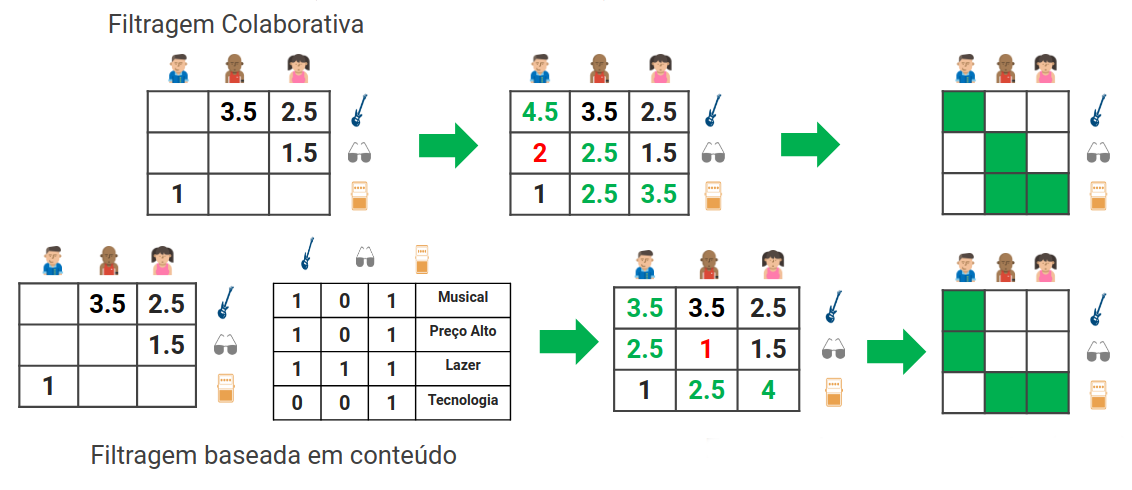
\includegraphics[width=1\linewidth]{imagens/hibridamista.png}
	\caption[Exemplo de filtragem híbrida mista]{Exemplo de filtragem híbrida mista, adaptado de \cite{araujo2011apprecommender}}
    \label{fig:algoritmohibridomisto}
\end{figure}

Para abordagem ponderada, é realizado uma normalização e combinação linear dos dados obtidos nas abordagens colaborativa e baseada em conteúdo, para que então, a partir disso, seja gerado a matriz de recomendação final. Nesse trabalho foi utilizado a média entre valores para o processo de combinação dos resultados, é possível ver um exemplo dessa abordagem na figura \ref{fig:algoritmohibridoponderado}:

\begin{figure}[H]
	\centering
	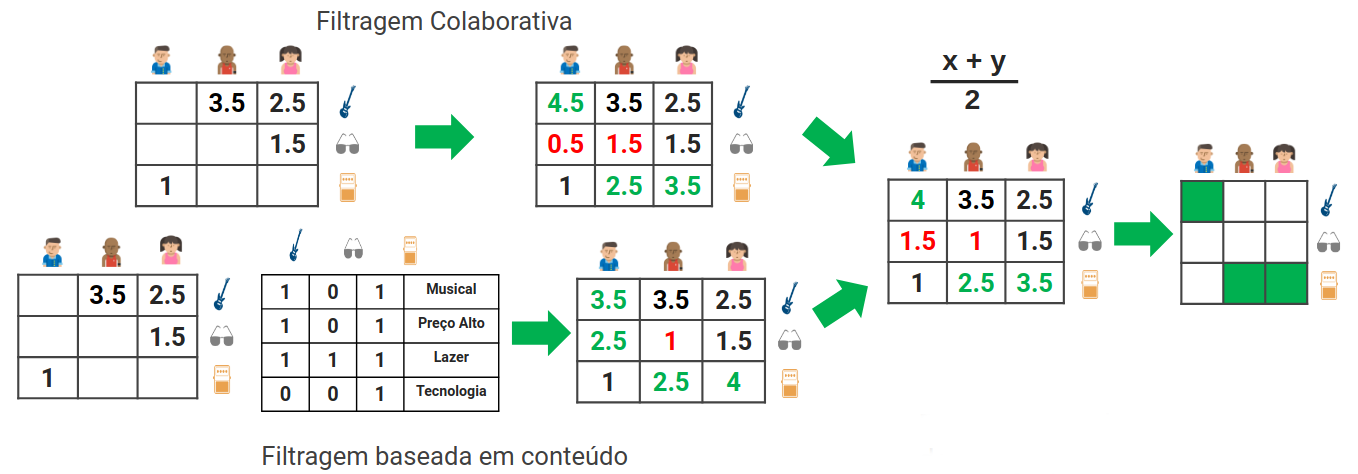
\includegraphics[width=1\linewidth]{imagens/hibridaponderada.png}
	\caption[Exemplo de filtragem híbrida ponderada]{Exemplo de filtragem híbrida ponderada, adaptado de \cite{araujo2011apprecommender}}
    \label{fig:algoritmohibridoponderado}
\end{figure}